
% !TeX spellcheck = en

\chapter{Introduction to Liquibase}
\section{Overview}
\marginpar{Overview \cite{Liquibase}}%
The Liquibase tool is a database schema change management solution that enables fast and safe database change releases from development to production. Liquibase \cite{Liquibase} will help to:

\begin{itemize}
	\item Control database schema changes for specific versions.
	\item Eliminate errors and delays when releasing databases.
	\item Automatically order scripts for deployment.
	\item Easily rollback changes.
	\item Collaborate with already used tools.
\end{itemize}

\marginpar{Support \cite{Liquibase}}%
Additionally, Liquibase works with over 50 databases categorized on different verification levels. Table \ref{tab:IntroductionToLiquibase:DBVerificationLevels}

\begin{table}[H]
	\centering
	\ra{1.3}
	\begin{tabularx}{\textwidth}{ll} 
		\toprule
		Verification Level & Description \\ 
		\midrule
		Guaranteed & \makecell[l]{Database tested and certified by Liquibase and works with all\\ Liquibase Pro capabilities.} \\[10pt]
		Foundational & \makecell[l]{Database tested and certified by Liquibase with the full set of\\ open source capabilities. Liquibase Pro functionality is not\\ guaranteed.} \\[15pt]
		Compatible & \makecell[l]{Widely reported as working by the community but has incomplete\\ functionality. Best effort support provided by Liquibase.} \\[10pt]
		Unverified & \makecell[l]{Not enough information for assessment. Best effort support\\ provided through community forums.} \\
		\bottomrule
	\end{tabularx}
	\caption{Supported Database, Verification Levels}
	\label{tab:IntroductionToLiquibase:DBVerificationLevels}
\end{table}

\marginpar{Pricing and Editions \cite{Liquibase}}%
Liquibase \cite{Liquibase} comes in three editions with different pricing: Free, Pro and Enterprise. Each edition adds more functionality than the preceding. However, the free, open-source version provides all the core functionalities needed. The Pro and Enterprise version targets larger teams with ten or more members. 

\marginpar{Community}%
Stars on GitHub: 3'600 (27. December 2022)\\
Tags on StackOverflow: 3,530 (27. December 2022)\\

\section{Functionality}
\marginpar{Organisation \cite{Liquibase}}%
Liquibase uses a changelog file to list database changes sequentially. Each change is defined in the changeset format and contains change types, which specify the operations to apply. Figure \ref{fig:IntroductionToLiquibase:LiquibaseChangelogStructure} shows this structure. Next to the changelog file is a property file, which specifies the database connection and additional parameters.

\begin{figure}[H]
	\centering
	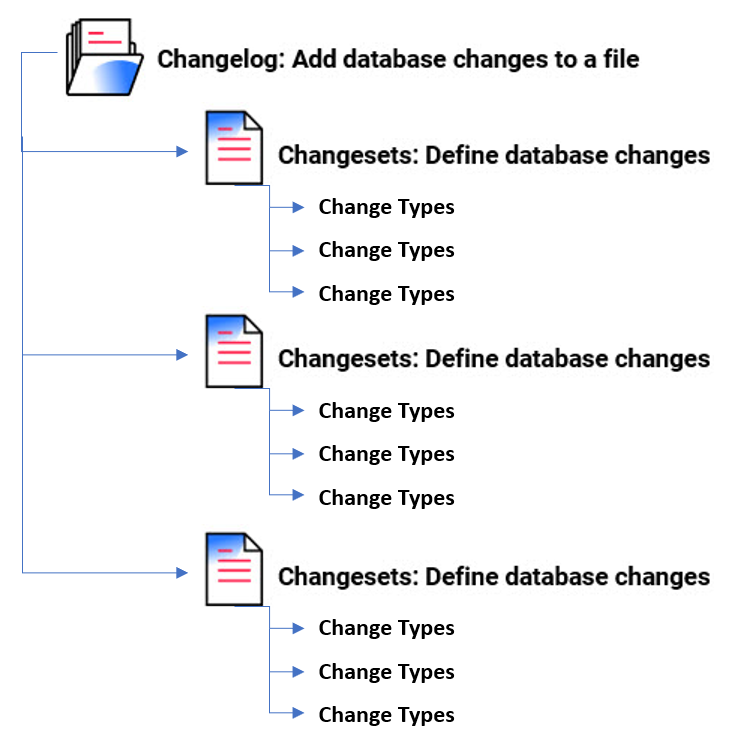
\includegraphics[width=0.65\textwidth]{./chapters/intro_liquibase/images/changelog-structure.png}
	\caption[Liquibase Organisation - Source: \cite{Liquibase}]{Liquibase Organisation}
	\label{fig:IntroductionToLiquibase:LiquibaseChangelogStructure}
\end{figure}

The workflow of Liquibase is shown in Figure \ref{fig:IntroductionToLiquibase:Workflow}. The workflow consists of creating changesets and adding them to the changelog file. Followed by the application of the update to the database. 

\marginpar{Workflow \cite{Liquibase}}%
\begin{figure}[H]
	\centering
	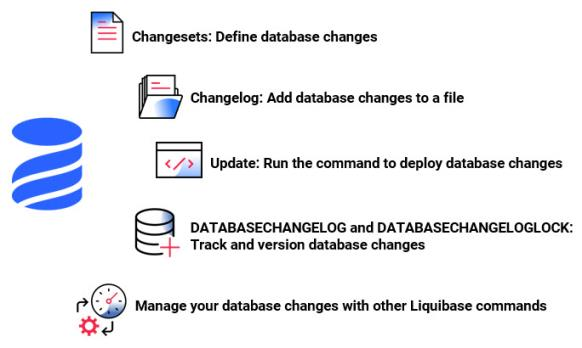
\includegraphics[width=0.95\textwidth]{./chapters/intro_liquibase/images/how-liquibase-works-general.jpg}
	\caption[Liquibase Workflow - Source: \cite{Liquibase}]{Liquibase Workflow}
	\label{fig:IntroductionToLiquibase:Workflow}
\end{figure}

The database changelog and database changeloglock table are created together with the first migration. The changelog table tracks deployed changes and ensure that only new changes are deployed.
The database changelog lock table prevents multiple instances of Liquibase updating the database.

\marginpar{Formats \cite{LiquibaseBlogXML}}%
Liquibase allows the definition of changesets in four different formats. They can either be written in SQL or XML, YAML and JSON. In comparison, the latter provides much more flexibility and features than SQL. Liquibase emphasizes the use of XML, YAML or JSON format for changelog files. As stated in their blog: "The magic happens when you use XML" \cite{LiquibaseBlogXML}.

\begin{figure}[H]
	\centering
	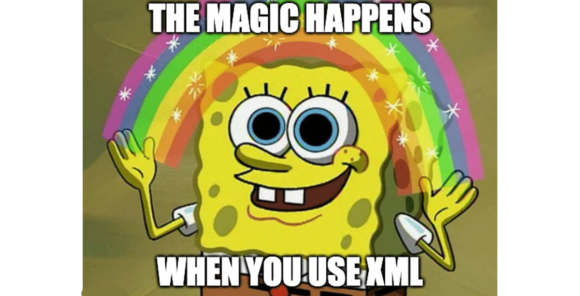
\includegraphics[width=0.65\textwidth]{./chapters/intro_liquibase/images/xml-magic.png}
	\caption[Liquibase, The Magic Happens when you use XML - Source: \cite{LiquibaseBlogXML}]{Liquibase, The Magic Happens when you use XML}
	\label{fig:IntroductionToLiquibase:Magic}
\end{figure}

By using the database-agnostic way of defining the changeset you gain the benefits of auto rollback, powerful change types, cross-platform compatibility and easy unit testing. The use of agnostic formats does not limit the use of \gls{SQL} changesets. Both can be used simultaneously. Using agnostic format for the majority of changes and use platform specific \gls{SQL} for the rest.


\section{Main Commands \cite{Liquibase}}
Liquibase categorizes the commands into six types: update, rollback, snapshot, diff, status and utility. The following paragraph provide a short description of each type.

\textbf{Update}\\
\marginpar{Update}%
The update command type includes a variety of commands to update the changes to the database. Important commands are update-count and validate. Update-count applies the next number of changesets indicated by the count variable. This function gives a lot of control. Validate checks the changelog for errors and is useful for debugging.

\textbf{Rollback}\\
\marginpar{Rollback}%
The rollback command type includes all commands to rollback applied changes to the database. The main command used is the rollback-count, which roll-backs the specified amount of changesets.

\textbf{Snapshot}\\
\marginpar{Snapshot}%
The snapshot command gathers the current database schema and compiles the results into \gls{CLI} or into a JSON file.

\textbf{Diff}\\
\marginpar{Diff}%
The diff command type allows different methods to compare two databases and even generate a changelog file which contains all differences as changesets.

\textbf{Status}\\
\marginpar{Satus}%
The status command lists all changesets that are not applied to the database. Useful for keeping track of deployed changes.


\section{Installation and Setup}
\marginpar{Installation \cite{Liquibase}}%
Liquibase provides an easy installation process on Windows, macOS and Linux.

\begin{minipage}[t]{0.5\textwidth}
	\textbf{Liquibase Clients}	
	\begin{itemize}
		\item \Gls{CLI}
		\item \gls{JAVAg} \acrshort{API}
	\end{itemize}
\end{minipage}
\begin{minipage}[t]{0.5\textwidth}
	\textbf{Third Party Plugins}
	\begin{itemize}
		\item Ant
		\item Maven
		\item Spring Boot.
	\end{itemize}
\end{minipage}
\vspace{0.3cm}

\marginpar{Setup \cite{Liquibase}}%
For the purpose of this seminar Liquibase was used through the \gls{CLI}. Setup a project with the following command: 

\begin{lstlisting}[language=bash]
liquibase init project
--project-dir=[path/to/some/directory]
--changelog-file=[file.ext]
--format=[sql|xml|json|yaml|yml]
--project-defaults-file=[liquibase.properties]
--url=[some/JDBC/URL]
--username=[string]
--password=[string]
\end{lstlisting}

Two separate projects were created for this seminar. One using YAML format and one using \gls{SQL} format otherwise identical.

\section{Best Practices}


\newpage